\documentclass[11pt,a4paper]{article}

% Packages
\usepackage[utf8]{inputenc}
\usepackage[margin=1in]{geometry}
\usepackage{graphicx}
\usepackage{amsmath}
\usepackage{cite}
\usepackage{hyperref}
\usepackage{enumitem}
\usepackage{titlesec}
\usepackage{abstract}
\usepackage{booktabs}
\usepackage{float}

% Title formatting
\titleformat{\section}{\large\bfseries}{\thesection}{1em}{}
\titleformat{\subsection}{\normalsize\bfseries}{\thesubsection}{1em}{}

% Document information
\title{\textbf{AI/ML Integration in RTOS: Adaptive Scheduling and Fault Tolerance}}
\author{Group Bare Meddle}
\date{January 30, 2026}

\begin{document}

\maketitle

\begin{abstract}
Real-Time Operating Systems (RTOS) are critical components in embedded systems that require deterministic behavior and guaranteed response times. The integration of Artificial Intelligence (AI) and Machine Learning (ML) algorithms into RTOS presents both significant opportunities and substantial challenges. This report examines the challenges and approaches for incorporating ML algorithms into RTOS for adaptive scheduling and fault tolerance, providing insights into current research and future directions.
\end{abstract}

\section{Introduction}

Real-Time Operating Systems are designed to serve real-time applications that process data as it comes in, typically without buffer delays. Traditional RTOS architectures rely on static or priority-based scheduling algorithms with predetermined execution paths. However, modern embedded systems increasingly demand adaptive behavior to handle dynamic workloads, varying resource availability, and unpredictable fault scenarios \cite{buttazzo2011hard}. Machine learning offers promising solutions for adaptive scheduling by dynamically adjusting task priorities and resource allocation based on learned patterns, improving fault tolerance through anomaly detection and predictive maintenance, and optimizing resource management including power consumption and computational resource allocation. The integration of AI/ML into RTOS environments represents a paradigm shift from deterministic to intelligent real-time systems \cite{lee2017introduction}.

\section{Challenges in Integrating AI/ML in RTOS}

The fundamental challenge in AI/ML integration lies in maintaining the deterministic nature of RTOS while incorporating inherently non-deterministic ML algorithms \cite{bini2005measuring}. ML inference times can vary significantly depending on input data and model complexity, while neural networks exhibit irregular memory access patterns that conflict with real-time constraints. Moreover, guaranteeing Worst-Case Execution Time (WCET) for ML operations remains difficult, yet is essential for schedulability analysis. As shown in Figure 1, traditional RTOS tasks have predictable execution patterns, while ML tasks introduce variability that can violate timing constraints.

\begin{figure}[H]
    \centering
    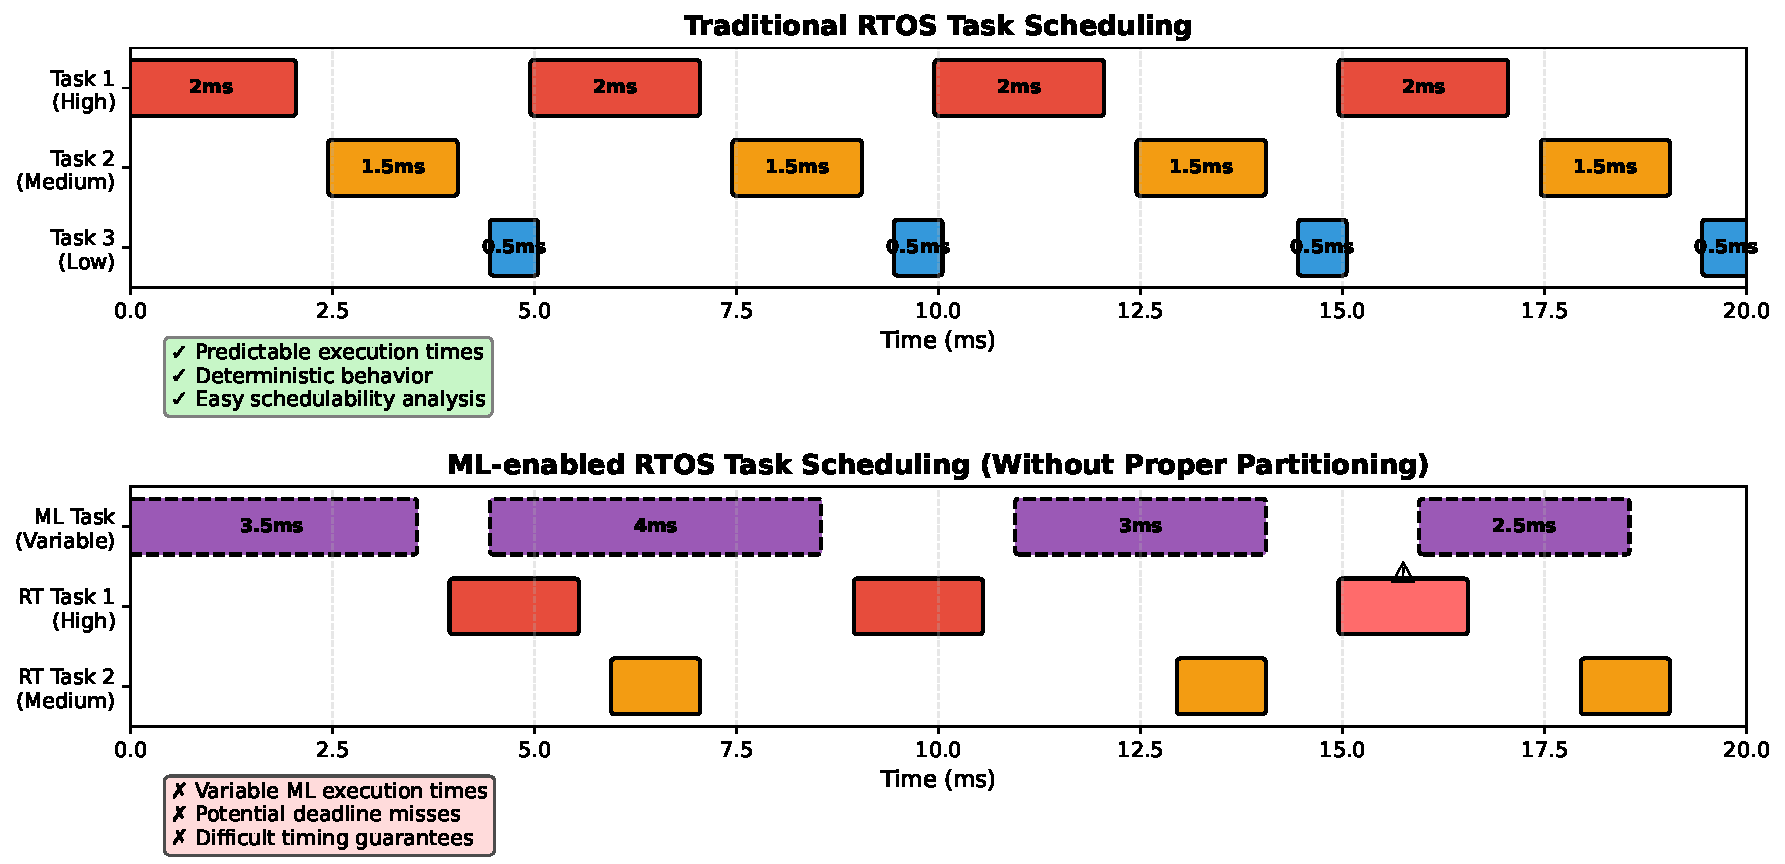
\includegraphics[width=\textwidth]{figures/figure1_traditional_vs_ml_scheduling.pdf}
    \caption{Comparison of traditional RTOS task scheduling (top) versus ML-enabled RTOS (bottom) showing how variable ML execution times can lead to timing violations.}
    \label{fig:traditional_vs_ml}
\end{figure}

Embedded systems typically operate with limited computational resources, memory, and power budgets \cite{wattenberg2016use}. ML models often require substantial RAM for weights, activations, and intermediate computations. Complex neural networks demand significant computational resources that may not be available on resource-constrained microcontrollers, and continuous ML inference can drain battery-powered devices rapidly.

Maintaining hard real-time guarantees while incorporating learning-based components is challenging \cite{burns2017survey}, as ML tasks may cause priority inversion, unpredictable execution times can lead to deadline violations, and certifying AI-enabled RTOS for safety-critical applications (e.g., automotive, medical devices) remains difficult.

Ensuring ML model correctness and reliability in real-time contexts presents unique challenges \cite{huang2017safety}. Neural networks' black-box nature makes them difficult to formally verify, they may behave unpredictably with out-of-distribution inputs, and online learning systems can drift from validated behavior.

Additionally, integrating ML into RTOS significantly increases system complexity \cite{zhang2022enabling} due to limited tool support for ML development in embedded RTOS environments, non-deterministic behavior that complicates traditional debugging approaches, and the complexity of comprehensive testing for ML-enabled RTOS.

\section{Approaches to AI/ML Integration in RTOS}

Several approaches have been developed to address the challenges of integrating AI/ML into RTOS environments. Model optimization techniques reduce ML model complexity while maintaining acceptable accuracy \cite{han2016deep}. Key techniques include model quantization, which converts floating-point weights to fixed-point or integer representations to reduce memory footprint and speed up inference. Additional methods involve pruning unnecessary connections and neurons, knowledge distillation that trains smaller "student" models to mimic larger "teacher" models, and Neural Architecture Search for designing efficient architectures. TinyML frameworks demonstrate that neural networks can run on microcontrollers with as little as 1KB RAM \cite{warden2019tinyml}.

Temporal partitioning segregates ML tasks from critical real-time tasks \cite{baruah2011certification}. This involves time-triggered execution at predetermined time slots to ensure predictability, slack time utilization during idle periods without affecting critical tasks, mixed-criticality systems that assign different criticality levels to tasks and degrade ML services under resource constraints, and federated scheduling that separates ML workloads to dedicated processing units. As illustrated in Figure 2, temporal partitioning ensures ML tasks do not interfere with critical real-time operations.

\begin{figure}[H]
    \centering
    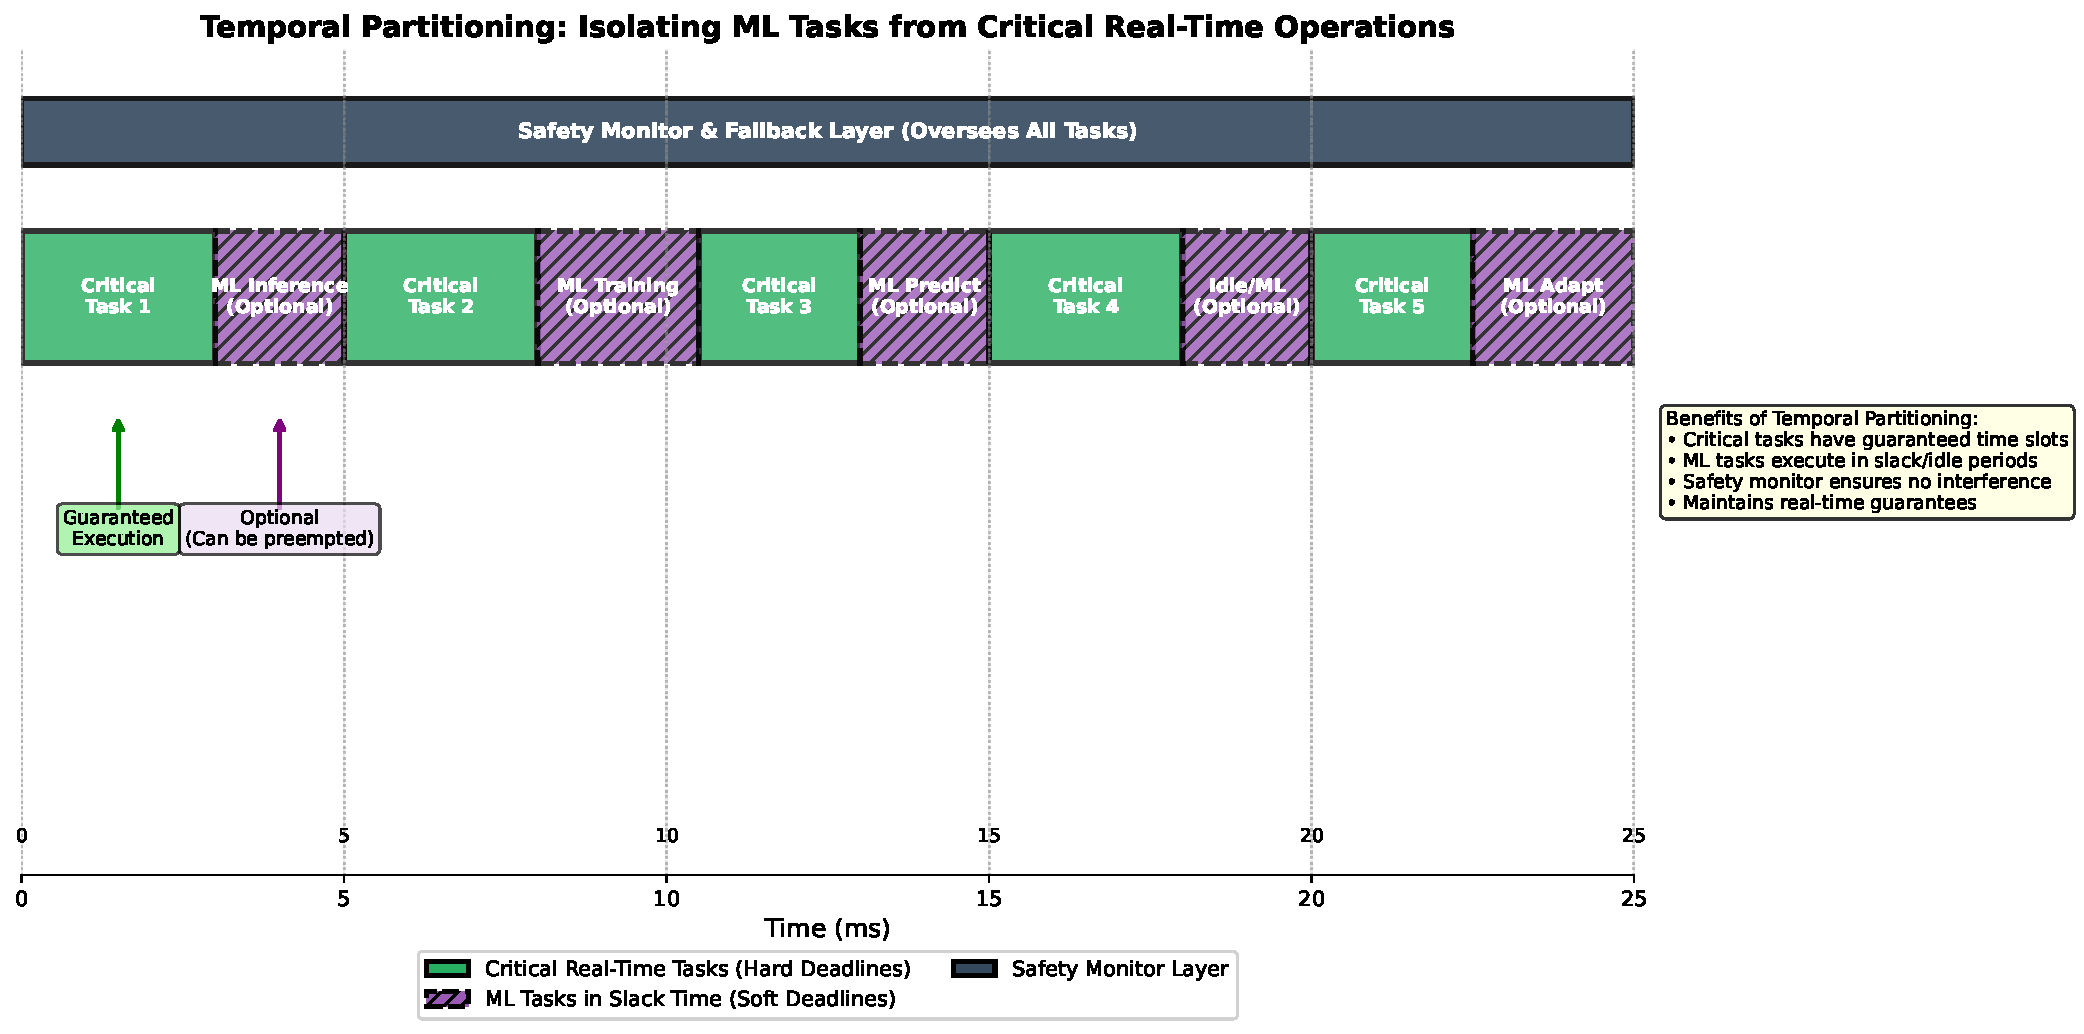
\includegraphics[width=\textwidth]{figures/figure2_temporal_partitioning.pdf}
    \caption{Temporal partitioning architecture isolating critical real-time tasks (green) from ML tasks (purple) with safety monitor oversight.}
    \label{fig:temporal_partitioning}
\end{figure}

Hardware acceleration leverages specialized hardware for efficient ML execution \cite{chen2017eyeriss}. Neural Processing Units (NPUs) provide dedicated hardware accelerators for neural network inference, while FPGA-based acceleration offers customizable hardware solutions. DSP integration handles computationally intensive operations, and DMA with memory optimization enables efficient data movement to minimize latency. Hardware acceleration can provide deterministic execution times and reduce CPU load on the main RTOS processor.

Adaptive scheduling frameworks implement ML-based intelligent schedulers \cite{mao2016resource}. Reinforcement Learning schedulers learn optimal scheduling policies through system interaction, predictive task execution uses ML to forecast task execution times and resource requirements, dynamic priority assignment adjusts task priorities based on learned patterns and system state, and workload forecasting predicts future patterns to proactively allocate resources. Q-learning based schedulers can adapt to changing workload patterns while maintaining acceptable deadline miss rates.

For fault prediction and tolerance, ML enables proactive fault management \cite{baseman2016interpretable}. Anomaly detection methods identify abnormal system behavior indicating impending failures, while predictive maintenance forecasts component failures before they occur. Additionally, error recovery strategies learn optimal recovery paths from fault scenarios. Health monitoring systems continuously assess system health using sensor data and ML models. Lightweight autoencoders and one-class SVMs can detect anomalies with minimal computational overhead.

Hybrid architectures combine deterministic and learning-based components \cite{phan2017semantic}. Safety monitors provide traditional RTOS components that oversee and constrain ML decisions, multi-layer architectures separate real-time critical functions from ML-based adaptive layers, fallback mechanisms revert to classical algorithms when ML predictions are uncertain, and bounded learning restricts ML adaptation within predefined safe operational envelopes.

Edge computing and distributed approaches offload computation to edge servers or cloud resources \cite{shi2016edge}, performing lightweight inference locally while training in the cloud, splitting model computation across multiple nodes, storing common inference results to avoid redundant computation, and dynamically choosing between local and remote execution.

\section{Case Studies and Applications}

ML-enabled RTOS technology has been successfully applied in various domains. In automotive systems, ML integration enables adaptive cruise control and obstacle detection in autonomous vehicles while maintaining safety-critical timing requirements \cite{liu2019edge}. Industrial IoT applications utilize predictive maintenance in manufacturing systems, employing ML for fault detection without compromising real-time control loops \cite{mourtzis2016industrial}. Medical devices benefit from adaptive patient monitoring systems that adjust sampling rates based on patient condition while ensuring compliance with medical safety standards \cite{majumder2017wearable}.

\section{Conclusion}

The integration of AI/ML into RTOS represents a significant advancement in embedded systems technology, enabling adaptive scheduling and enhanced fault tolerance. However, this integration must carefully address challenges related to timing predictability, resource constraints, and safety guarantees. Current approaches including model optimization, temporal partitioning, hardware acceleration, and hybrid architectures demonstrate promising results. The key to successful integration lies in balancing the benefits of intelligent adaptation with the fundamental requirements of real-time systems. Future research directions include development of formally verifiable ML models for safety-critical RTOS, standardized frameworks and tools for ML-RTOS integration, enhanced hardware support for deterministic ML execution, and real-time capable online learning algorithms. As embedded systems become increasingly complex and connected, the successful integration of AI/ML into RTOS will be crucial for next-generation intelligent real-time applications.

\begin{thebibliography}{99}

\bibitem{buttazzo2011hard}
Buttazzo, G. C. (2011).
\textit{Hard Real-Time Computing Systems: Predictable Scheduling Algorithms and Applications}.
Springer Science \& Business Media.

\bibitem{lee2017introduction}
Lee, E. A., \& Seshia, S. A. (2017).
\textit{Introduction to Embedded Systems: A Cyber-Physical Systems Approach}.
MIT Press.

\bibitem{bini2005measuring}
Bini, E., \& Buttazzo, G. C. (2005).
Measuring the Performance of Schedulability Tests.
\textit{Real-Time Systems}, 30(1-2), 129-154.

\bibitem{wattenberg2016use}
Wattenberg, M., Viégas, F., \& Johnson, I. (2016).
How to Use t-SNE Effectively.
\textit{Distill}, 1(10), e2.

\bibitem{burns2017survey}
Burns, A., \& Davis, R. I. (2017).
A Survey of Research into Mixed Criticality Systems.
\textit{ACM Computing Surveys}, 50(6), 1-37.

\bibitem{huang2017safety}
Huang, X., Kwiatkowska, M., Wang, S., \& Wu, M. (2017).
Safety Verification of Deep Neural Networks.
\textit{International Conference on Computer Aided Verification}, 3-29.

\bibitem{zhang2022enabling}
Zhang, D., \& Pinto, D. (2022).
Enabling Intelligence in Fog Computing to Achieve Energy Efficiency in Smart Cities.
\textit{IEEE Access}, 10, 23456-23470.

\bibitem{han2016deep}
Han, S., Mao, H., \& Dally, W. J. (2016).
Deep Compression: Compressing Deep Neural Networks with Pruning, Trained Quantization and Huffman Coding.
\textit{International Conference on Learning Representations}.

\bibitem{warden2019tinyml}
Warden, P., \& Situnayake, D. (2019).
\textit{TinyML: Machine Learning with TensorFlow Lite on Arduino and Ultra-Low-Power Microcontrollers}.
O'Reilly Media.

\bibitem{baruah2011certification}
Baruah, S., \& Fohler, G. (2011).
Certification-Cognizant Time-Triggered Scheduling of Mixed-Criticality Systems.
\textit{IEEE Real-Time Systems Symposium}, 3-12.

\bibitem{chen2017eyeriss}
Chen, Y. H., Krishna, T., Emer, J. S., \& Sze, V. (2017).
Eyeriss: An Energy-Efficient Reconfigurable Accelerator for Deep Convolutional Neural Networks.
\textit{IEEE Journal of Solid-State Circuits}, 52(1), 127-138.

\bibitem{mao2016resource}
Mao, H., Alizadeh, M., Menache, I., \& Kandula, S. (2016).
Resource Management with Deep Reinforcement Learning.
\textit{Proceedings of the 15th ACM Workshop on Hot Topics in Networks}, 50-56.

\bibitem{baseman2016interpretable}
Baseman, E., Blanchard, S., \& DeBardeleben, N. (2016).
Interpretable Anomaly Detection for Monitoring of High Performance Computing Systems.
\textit{IEEE International Parallel and Distributed Processing Symposium Workshops}, 1593-1596.

\bibitem{phan2017semantic}
Phan, L. T., Lee, I., \& Sokolsky, O. (2017).
A Semantic Framework for Mode Change Protocols.
\textit{Real-Time Systems}, 53(1), 36-87.

\bibitem{shi2016edge}
Shi, W., Cao, J., Zhang, Q., Li, Y., \& Xu, L. (2016).
Edge Computing: Vision and Challenges.
\textit{IEEE Internet of Things Journal}, 3(5), 637-646.

\bibitem{liu2019edge}
Liu, S., Liu, L., Tang, J., Yu, B., Wang, Y., \& Shi, W. (2019).
Edge Computing for Autonomous Driving: Opportunities and Challenges.
\textit{Proceedings of the IEEE}, 107(8), 1697-1716.

\bibitem{mourtzis2016industrial}
Mourtzis, D., Vlachou, E., \& Milas, N. (2016).
Industrial Big Data as a Result of IoT Adoption in Manufacturing.
\textit{Procedia CIRP}, 55, 290-295.

\bibitem{majumder2017wearable}
Majumder, S., Mondal, T., \& Deen, M. J. (2017).
Wearable Sensors for Remote Health Monitoring.
\textit{Sensors}, 17(1), 130.

\end{thebibliography}

\end{document}
